\vspace{1cm}
\fancyhead[C]{\normalsize\textbf{$\qquad$ Teil I: Offene Aufgaben}}
\renewcommand{\labelenumi}{\theenumi.}
\section*{Aufgabe 1 (36 Punkte)}
\vspace{0.4cm}
\section*{Aufgabe 1 (36 Punkte)}
\vspace{0.4cm}
%\titleformat{\subsection}[runin]
%{\normalfont\large\bfseries}{\thesubsection}{1em}{}
\subsection*{\aufgabe{a1}{6}} 
Thomas Robert Malthus (1766-1834), ein britischer Ökonom und Pfarrer, veröffentlichte
1798 seinen vielbeachteten \textit{Essay on the Principle of Population}.
Er formulierte das Axiom, dass die Weltbevölkerung exponentiell wachse, die Nahrung dagegen nur linear. 
Das bedeutet, dass die Funktion $ n(t) $, welche die Anzahl Menschen angibt, die man bei optimaler Verteilung der zur Verfügung stehenden Nahrungsmittel zu Zeit $ t $ ernähren könnte, eine lineare ist:
\begin{align*}
	n(t) = a + b \cdot t.
\end{align*}
Die Weltbevölkerung $ w(t) $ betrug im Jahre 1800 ($ t= 0 $) rund eine Milliarde, d.h. $ w(0) = 10^9 $.
Wir wollen annehmen, dass die Weltbevölkerung rund $ 1\% $ pro Jahr wächst.
Außerdem wollen wir mit
\begin{align*}
	a = 2 \cdot 10^9 \ \textrm{und} \ b = 0.2 \cdot 10^9
\end{align*}
rechnen.
\begin{description}
	\item[Beweisen Sie:] 
	Es gibt genau einen Zeitpunkt $ t^\star > 400 $, an dem die Weltbevölkerung gerade noch ernährt werden kann, d.h., für $ w(t^\star)  = n(t^\star )$ ist.
\end{description}  
\
\\
\textbf{Lösung:}
\begin{mdframed}
\underline{\textbf{Vorgehensweise:}}
\renewcommand{\labelenumi}{\theenumi.}
\begin{enumerate}
\item 

\end{enumerate}
\end{mdframed}
\underline{1. }\\

 


\newpage

\subsection*{\aufgabe{a2}{6}}
Thomas Robert Malthus (1766-1834), ein britischer Ökonom und Pfarrer, veröffentlichte
1798 seinen vielbeachteten \textit{Essay on the Principle of Population}.
Er formulierte das Axiom, dass die Weltbevölkerung exponentiell wachse, die Nahrung dagegen nur linear. 
Das bedeutet, dass die Funktion $ n(t) $, welche die Anzahl Menschen angibt, die man bei optimaler Verteilung der zur Verfügung stehenden Nahrungsmittel zu Zeit $ t $ ernähren könnte, eine lineare ist:
\begin{align*}
	n(t) = a + b \cdot t.
\end{align*}
Die Weltbevölkerung $ w(t) $ betrug im Jahre 1800 ($ t= 0 $) rund eine Milliarde, d.h. $ w(0) = 10^9 $.
Wir wollen annehmen, dass die Weltbevölkerung rund $ 1\% $ pro Jahr wächst.
Außerdem wollen wir mit
\begin{align*}
	a = 2 \cdot 10^9 \ \textrm{und} \ b = 0.2 \cdot 10^9
\end{align*}
rechnen.\\
\\
Es gibt genau einen Zeitpunkt $ t^\star > 400 $, an dem die Weltbevölkerung gerade noch ernährt werden kann, d.h., für $ w(t^\star)  = n(t^\star )$ ist.\\
\\
Verwenden Sie eine Taylor-Approximation zweiter Ordnung im Punkt $ t_0 = 400 $, um eine Näherung für $ t^\star $ zu finden.
\\ \\
\textbf{Lösung:}
\begin{mdframed}
\underline{\textbf{Vorgehensweise:}}
\renewcommand{\labelenumi}{\theenumi.}
\begin{enumerate}
\item 
\end{enumerate}
\end{mdframed}

\underline{1. }\\


\newpage
\subsection*{\aufgabe{b}{10}}
Max hat über seine Verhältnisse gelebt. 
Deshalb hat er nun Schulden von mehreren hunderttausend Franken.
Die Schuldenberatung vermittelt ihm am Anfang des Jahres einen Privatkredit mit $ i = 5 \% $ in der genannten Höhe von $ S = 355'000 \ [\textrm{CHF}] $, den er in $ 12 $ gleich grossen Raten $ C $ jeweils per Jahresende abbezahlen muss. 
\begin{enumerate}
	\item[(b1)] Fügen Sie die Ereignisse und Mittelflüsse dem Zeitstrahl hinzu.
	\item[(b2)] Berechnen Sie die Höhe der Ratenzahlung $ C $.
\end{enumerate}
Am Ende des vierten Jahres gewinnt Max im Lotto CHF $ 160'000 $.
Er beschließt in diesem Jahr statt der normalen Rate $ C $ den ganzen Lottogewinn zur Abzahlung des Kredits zu benützen.
\begin{enumerate}
	\item[(b3)] Ergänzen Sie die Information am Zeitstrahl und berechnen Sie die Restschuld $ \overline{S} $ nach der Einzahlung am Ende des vierten Jahres.
\end{enumerate}
Max zahlt nun weiter am Ende jeden Jahres den Betrag $ C $ zu Tilgung seiner Restschuld $ \overline{S} $.
\begin{enumerate}
	\item[(b4)] Wie viele Zahlungen muss er machen, bis er die Restschuld vollkommen getilgt hat?
	\item[(b5)] Mit der letzten Rate muss nicht mehr der komplette Betrag $ C $ geleistet werden. Wie hoch ist die Zahlung genau?
\end{enumerate}
\begin{center}
	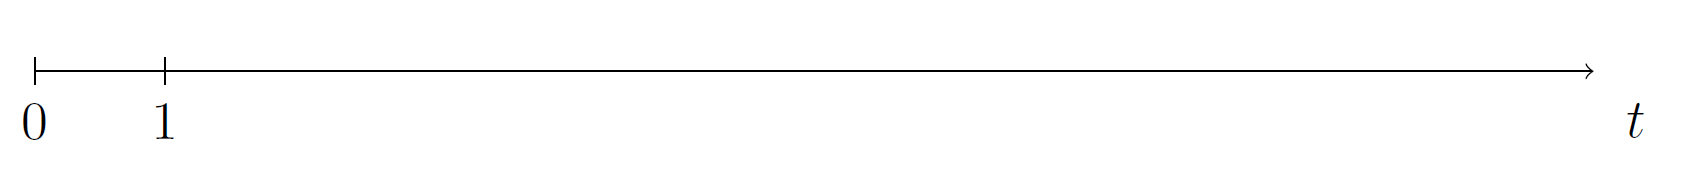
\includegraphics[scale=0.3]{pictures/zeitstrahl_1_b}
\end{center}
\ \\
\textbf{Lösung:}
\begin{mdframed}
\underline{\textbf{Vorgehensweise:}}
\begin{enumerate}
\item 
\end{enumerate}
\end{mdframed}

\underline{1. }\\



\newpage
\subsection*{\aufgabe{c}{6}}
Nach der Relativitätstheorie gilt für die Masse $ m $ eines Körpers, der sich mit der Geschwindigkeit $ v $ bewegt
\begin{align*}
	m(v)
	=
	\frac{m_0}{\sqrt{1 - \frac{v^2}{c^2}}}.
\end{align*}
Dabei ist $ c $ die Lichtgeschwindigkeit $ (299'792'458 \nicefrac{m}{s}) $ und $ m_0 $ die Masse in Ruhe.
\begin{enumerate}
	\item[(c1)] Berechnen Sie die Elastizität $ \varepsilon_m $ von $ m(v) $.
	\item[(c2)] Um wie viel Prozent ändert sich näherungsweise die Masse, wenn die Geschwindigkeit von $ v_0 = 0.5c $ um $ 5 \% $ erhöht wird?
\end{enumerate}
\ \\
\textbf{Lösung:}
\begin{mdframed}
\underline{\textbf{Vorgehensweise:}}
\begin{enumerate}
\item 
\end{enumerate}
\end{mdframed}

\underline{1.}\\


\newpage
\subsection*{\aufgabe{c}{10}}
Eine Familie leiht sich CHF $ 1'000'000 $, um ein Haus zu kaufen.
Der Zins beträgt zu Beginn $ i = 1 \% $.
Die Familie beschliesst, CHF $ C_1 $ am Ende jeden Jahres für $ 10 $ Jahre zurückzuzahlen, um so den Schuldenstand auf CHF $ 750'000 $ am Ende des $ 10. $ Jahres zu reduzieren.
Am Ende des $ 5 $-ten Jahres ergibt sich die Möglichkeit einer Sondertilgung.
Die Familie zahlt folglich am Ende des $ 5 $-ten Jahres einen Gesamtbetrag von CHF $ 150'000 $ (einschliesslich $ C_1 $) zurück und verhandelt die Konditionen mit der Bank neu.
Der Zinssatz fällt damit auf $ 0.5 \% $.
Die Familie beschliesst, die Schulden weiterhin mit CHF $ C_1 $ am Ende jeden Jahres zurückzuzahlen, bis diese auf CHF $ 500'000 $ reduziert sind.
Aus steuerlichen Gründen zahlen sie anschliessend CHF $ C_2 $ pro Jahr an die Bank,
um ihre Schulden konstant bei CHF $ 500'000 $ zu halten.
\begin{enumerate}
	\item[(c1)]
	Fügen Sie alle Ereignisse und Mittelflüsse dem Zeitstrahl hinzu.
	\item[(c2)] 
	Berechnen Sie $ C_1 $.
	\item[(c3)] Wie hoch ist der Schuldenstand, nachdem die Familie die Zahlung von CHF 150'000 am Ende des $ 5 $-ten Jahres veranlasst hat?
	\item[(c4)] 
	Wie lange dauert es nach Ende des $ 5 $-ten Jahres, bis der Schuldenstand CHF $ 500'000 $ erreicht hat?
	\item[(c5)]
	Berechnen Sie $ C_2 $.
\end{enumerate}
\begin{center}
	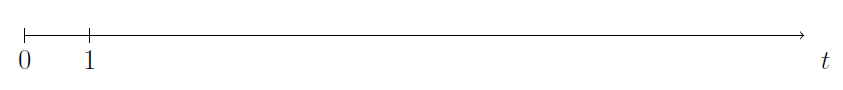
\includegraphics[scale=0.6]{pictures/zeitstrahl_1_c}
\end{center}
\ \\
\textbf{Lösung:}
\begin{mdframed}
	\underline{\textbf{Vorgehensweise:}}
	\begin{enumerate}
		\item[(c1)] Erstelle den Zeitstrahl.
		\item[(c2)] Berechne die jährliche Zahlung $ C_1 $.
		\item[(c3)] Bestimme den Schuldenstand nach der Sondertilgung.
		\item[(c4)] Bestimme die Anzahl an Jahren um einen Schuldenstand von $ 500'000 $ zu erreichen.
		\item[(c5)] Bestimme die Rate $ C_2 $ für einen konstanten Schuldenstand.
	\end{enumerate}
\end{mdframed}

\newpage
\underline{(c1) Erstelle den Zeitstrahl}\\
Der Zeitstrahl ist durch
\begin{center}
	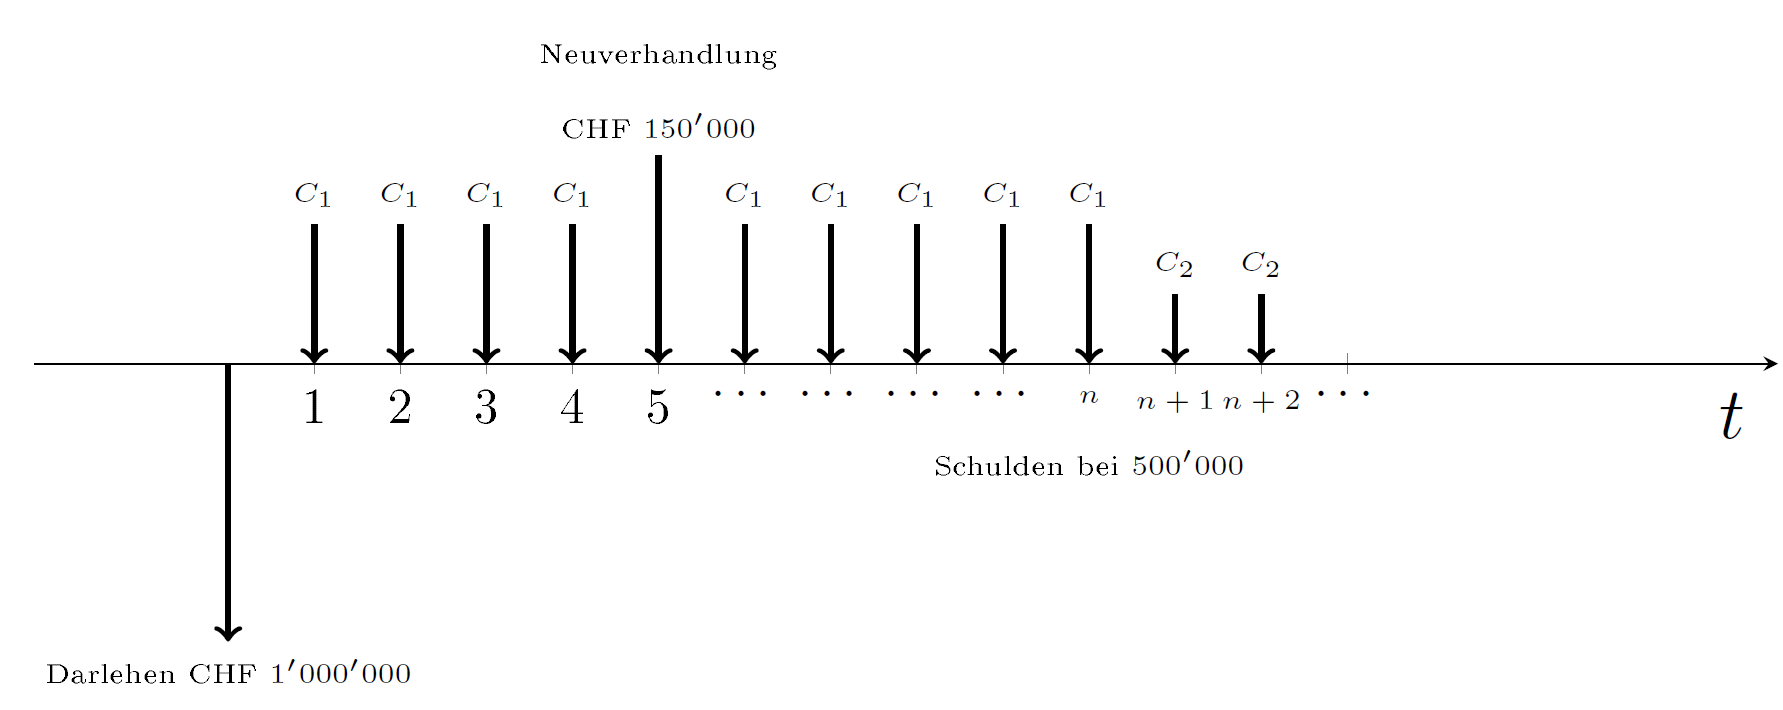
\includegraphics[scale=0.35]{pictures/zeitstrahl_1_c_filled}
\end{center}
gegeben. Damit ist die Teilaufgabe (c1) erledigt\\
\\
\underline{(c2) Berechne die jährliche Zahlung $ C_1 $}\\
Es war geplant, $ C_1 $ am Ende jeden Jahres über $ 10   $ Jahre zurückzuzahlen, sodass die Schulden von $ 1'000'000 $ CHF auf $ 750'000 $ reduziert werden.
Bei einem Zinssatz von $ 1\% $ ist ihm Jahre $ 10  $ der Betrag
\begin{align*}
	1'000'000(1+ 1 \%)^{10} - 750'000
	=
	1'000'000 \cdot 1.01^{10} -750'000
	\approx
	354'622.10
\end{align*}
zur Reduktion der Schulden notwendig. Dieser Wert muss nun einer nachschüssigen Rente mit jährlicher Zahlung $ C_1 $ nach $ 10 $ Jahren entsprechen.
Mit dem Endwert einer nachschüssigen Rente nach $ 10 $ Jahren erhalten wir:
\begin{align*}
	C_1 \frac{(1+ 1 \%)^{10}  - 1}{1 \%} = 354'622.10
	\
	\Leftrightarrow 
	\
	C_1 = \frac{1 \%}{(1+ 1 \%)^{10}  - 1} \cdot 354'622.10
	\approx 33'895.50 \ \mathrm{(CHF)}.
\end{align*}
Damit müssen jährlich ca. $ 33'895.50 $ CHF zurückgezahlt werden.\\
\\
\underline{(c3) Bestimme den Schuldenstand nach der Sondertilgung}\\
Den Schuldenstand nach $ 5  $ Jahren erhalten wir aus der über $ 5 $ Jahre verzinsten Kreditsumme abzüglich der über $ 5 $ Jahre getätigten Rückzahlung(Endwert nach $ 5 $ Zahlungen von $ C_1 $) und abzüglich 
der Sondertilgung $ 150'000 - C_1 $ CHF im fünften Jahr. Man beachte das einschliesslich in der Aufgabenstellung.
Damit ergibt sich für den Schuldenstand am Ende des fünften Jahres:
\begin{align*}
	&\underbrace{1'000'000(1+1 \%)^{5}}_{\textrm{Kreditsumme über } 5 \textrm{ Jahre verzinst}}
	-
	\underbrace{C_1 \frac{(1+ 1 \%)^{5}  - 1}{1 \%}}_{
	\textrm{Endwert nach $ 5 $ Jahren}
	}
	-
	\underbrace{(150'000 - C_1)}_{\textrm{Sondertilgung}}\\
	&\approx 1'051'010
	- 33'895.5 \frac{(1+ 1\%)^5 - 1}{1 \%} -150'000 + 33'895.5\\
	&\approx
	1'051'010
	-
	172'901.1
	-150'000 + 33'895.5\\
	&= 
	762'004.4 \ \textrm{(CHF)}.
\end{align*}
Am Ende des fünften Jahres hat die Familie eine Restschuld von $ 762'004.4 $ CHF.\\
\\
\newpage
\underline{(c4) Bestimme die Anzahl an Jahren um einen Schuldenstand von $ 500'000$ zu erreichen}\\
Nun ist die Frage nach wie vielen Jahren der Schuldenstand von $ 762'004.4 $ CHF auf 
$ 500'000 $ CHF sinkt.
Hierbei ist der neue Zinssatz durch $ i = 0.5 \% $ und die Jahresrate bleibt $ C_1 $.
Damit erhalten wir die Gleichung:
\begin{align*}
	\underbrace{500'000}_{\textrm{Zielschuldenstand}}
	&=
	\underbrace{762'004.4 (1+ 0.5 \%)^n}_{\textrm{Verzinsung über $ n $ Jahre}}
	-
	\underbrace{C_1 \frac{(1+ 0.5 \%)^{n}  - 1}{0.5 \%}}_{\textrm{Endwert nach $ n $ Jahren}}\\
	&=
	\left(762'004.4 - \frac{C_1}{0.5 \%} \right)(1+ 0.5 \%)^{n} + \frac{C_1}{0.5 \%}.
\end{align*}
Durch Auflösen der Gleichung nach $ n $ erhalten wir:
\begin{align*}
	&\left(762'004.4 - \frac{C_1}{0.5 \%} \right)(1+ 0.5 \%)^{n} = 500'000 -  \frac{C_1}{0.5 \%}\\
	\ \Leftrightarrow \
	&(1 + 0.5 \%)^n
	=
	\frac{500'000 -  \frac{C_1}{0.5 \%}}{762'004.4 - \frac{C_1}{0.5 \%}}\\
	\ \Leftrightarrow \
	&n  \ln(1 + 0.5 \%)
	=
	\ln\left(
	\frac{500'000 -  \frac{C_1}{0.5 \%}}{762'004.4 - \frac{C_1}{0.5 \%}}
	\right)
	= 
	\ln\left(500'000 -  \frac{C_1}{0.5 \%} \right)
	- 
	\ln\left(762'004.4 - \frac{C_1}{0.5 \%} \right)\\
	\ \Leftrightarrow \
	&n = 
	\frac{\ln\left(500'000 -  \frac{C_1}{0.5 \%} \right)
		- 
		\ln\left(762'004.4 - \frac{C_1}{0.5 \%} \right)}{\ln(1 + 0.5 \%)} \approx 8.54.
\end{align*}
Damit erreicht die Familie den Schuldenstand $ 9  $ Jahre nach der Sondertilgung bzw. dem Abschluss der neuen Konditionen.
Genau genommen ist die verbleibende Schuld nach $ 9 $ Jahren geringer als $ 500'000 $ CHF, denn es gilt:
\begin{align*}
	762'004.4 (1+ 0.5 \%)^9 - C_1 \frac{(1+ 0.5 \%)^{9}  - 1}{0.5 \%}
	\approx 485'756.1 \ \textrm{(CHF)}.
\end{align*}
Damit erhalten wir eine Interpretationsmöglichkeit, weswegen $ n = 8.54 $ und $ n  = 9 $ beides korrekte Antworten sind. In der nächsten Teilaufgabe rechnen wir mit einem Schuldenstand von $ 500'000 $ weiter.\\
\\
\underline{(c5) Bestimme die Rate $ C_2 $ für einen konstanten Schuldenstand}\\
Die Schulden von $ 500'000 $ bleiben konstant, wenn $ C_2 $ den anfallenden Zinsen entspricht. Also ist $ C_2 $ durch 
\begin{align*}
	C_2=  0.5 \% \cdot 500'000 = 2'500 \ \textrm{(CHF) }
\end{align*}
gegeben.\\
\\
Damit können sie als reicher Sack die Linkspartei für läppische $ 2'500 $ CHF verärgern, indem sie $ 2'500 $ CHF an dem Fiskus vorbeischleusen und diese stattdessen ihren Buddys von der Bank geben.
\newpage 

\subsection*{\aufgabe{d}{10}}
Ein Anbieter für Tablets schätzt die Nachfrage $ q_d $ nach seinem neusten Produkt auf
\begin{align*}
	q_d(p)
	=
	\frac{15'840 - 30 \ p}{p + 50},
\end{align*}
wobei $ p > 20  $ der Verkaufspreis in US-Dollar pro Tablet ist.
Die Kosten für Produktion und Vertrieb eines Tablets betragen $ 20  $ US-Dollar.
\begin{enumerate}
	\item[(d1)]
	Bestimmen Sie die Gewinnfunktion des Anbieters unter der Annahme, dass der Preis $ p > 20 $ ist.
	\item[(d2)]
	Leiten Sie die Funktion her, welche die Elastizität des Gewinns in Abhängigkeit vom Verkaufspreis beschreibt.
	\item[(d3)]
	Approximieren Sie mit Hilfe der Elastizitätsfunktion die relative Änderung des Gewinns bei einer Erhöhung des anfänglichen Verkaufspreises von $ p_0 = 100 $ US-Dollar um $ 5 $ US-Dollar.
\end{enumerate}

\ \\
\textbf{Lösung:}
\begin{mdframed}
	\underline{\textbf{Vorgehensweise:}}
	\begin{enumerate}
		\item[(d1)] Gebe die Gewinnfunktion an.
		\item[(d2)] Verwende einen Zusammenhang zwischen Kettenregel und der Logarithmusfunktion.
		\item[(d3)] Approximiere die relative Änderung durch die Elastizität.
	\end{enumerate}
\end{mdframed}

\underline{(d1) Gebe die Gewinnfunktion an}\\
Wir bezeichnen die Gewinnfunktion mit  $ G $. Diese Funktion besteht aus der Differenz aus Ertrag und Kosten. Mit $ E $ und $ K $ bezeichnen wir die Ertrags bzw. Kostenfunktion.
Damit gilt
\begin{align*}
	E(p) = q_d(p) \cdot p \ \textrm{und} \ K(p) = q_d(p) \cdot 20
\end{align*}
für $ p >20 $. 
Die Gewinnfunktion für $ p > 20 $ ergibt sich dann durch das Bilden der Differenz:
\begin{align*}
	G(p)
	= 
	E(p) -  K(p)
	=
	q_d(p) \cdot p - q_d(p) \cdot 20
	=
	q_d(p) \cdot (p -20)
	=
	\frac{15'840 - 30 \ p}{p + 50} (p -20).
\end{align*}
\ \\
\underline{(d2) Verwende einen Zusammenhang zwischen Kettenregel und der Logarithmusfunktion.}\\
Die Elastizität des Gewinns in Abhängigkeit des Preises $ p $ ist durch
\begin{align*}
	\varepsilon_{G}(p) = p \frac{G^\prime(p)}{G(p)}
\end{align*}
gegeben. Nun liegen zwei Möglichkeiten vor. Die Erste ist das (fehleranfällige) bestimmen der Ableitung von $ G $. Deswegen werden dies als Alternative durchführen.
Für die Zweite betrachten wir die aus der Kettenregel folgende Tatsache:
\begin{align*}
	(\ln(f(x)))^\prime = \frac{1}{f(x)} \cdot f^\prime(x)  = \frac{f^\prime(x)}{f(x)}.
\end{align*}
Wenn wir also die Ableitung von $ \ln(G(p))) $ bestimmen können, erhalten wir die Elastizität des Gewinns in Abhängigkeit des Preises $ p $ unmittelbar.
Hierfür formen wir zunächst $ \ln(G(p))) $ mit Logarithmusregeln um:
\begin{align*}
	\ln(G(p)))
	&=
	\ln \left(\frac{15'840 - 30  p}{p + 50} (p -20)\right)
	=
	\ln \left((15'840 - 30  p)(p -20) \frac{1}{p + 50}\right)\\
	&=
	\ln(15'840 - 30  p) + \ln(p -20) - \ln(p + 50).
\end{align*}
Damit vereinfacht sich das Differenzieren und  mit $\frac{30}{15'840} = \frac{1}{528}$ erhalten wir:
\begin{align*}
	(\ln(G(p))))^\prime
	&=
	(\ln(15'840 - 30 p) + \ln(p -20) - \ln(p + 50))^\prime
	=
	\frac{-30}{15'840 - 30 p} + \frac{1}{p -20} - \frac{1}{p + 50}\\
	&=
	\frac{1}{p - 528} + \frac{1}{p -20} - \frac{1}{p + 50}.
\end{align*}
Insgesamt ist die Elastizität durch
\begin{align*}
	\varepsilon_{G}(p) = p \frac{G^\prime(p)}{G(p)}
	= p \cdot 	(\ln(G(p))))^\prime 
	=
	\frac{p}{p - 528} + \frac{p}{p -20} - \frac{p}{p + 50}
\end{align*}
gegeben.\\
\\
Alternativ erhalten wir mit der Produkt-und Quotientenregel:
\begin{align*}
	G^\prime(p)
	&=
	\frac{(-30(p-20) + (15'840 - 30 p))(p+50) -(15'840 -30 p)(p-20) }{(p+50 )^2}\\
	&=
	\frac{-30(p-20)(p+50) + (15'840 - 30 p)(p+50- p + 20)}{(p+50 )^2}\\
	&=
	\frac{-30(p-20)(p+50) + 70 (15'840 - 30 p)}{(p+50 )^2}.
\end{align*}
Für die Elastizität folgt
\begin{align*}
	\varepsilon_{G}(p) = p \frac{G^\prime(p)}{G(p)}
	&=
	p \cdot \frac{-30(p-20)(p+50) + 70 (15'840 - 30 p)}{(p+50 )^2} \cdot 
	\frac{p +50}{(15'840 - 30 p)(p-20)}\\
	&=
	\frac{p}{p - 578} + \frac{70p}{(p+50)(p-20)}
\end{align*}
durch geschicktes Kürzen. Das dies der vorher bestimmten Elastizität entspricht lassen wir euch als (Bruchrechen-)Übungsaufgabe.\\
\\
\underline{(d3) Approximiere die relative Änderung durch die Elastizität}\\
Die relative Änderung von $ 100 $ USD auf $ 105 $USD des Gewinns ist durch 
\begin{align*}
	\frac{G(105) -G(100)}{G(100)}
\end{align*}
gegeben. Für diese gilt der Zusammenhang
\begin{align*}
	\frac{G(105) -G(100)}{G(100)}
	\approx
	\varepsilon_{G}(100) \frac{105- 100}{100} = \varepsilon_{G}(100) \cdot 5 \%
\end{align*}
mit der Elastizität.
Wegen 
\begin{align*}
	\varepsilon_{G}(100) = \frac{100}{100 - 528} + \frac{100}{100 - 20} - \frac{100}{100 + 50}
	\approx 0.35
\end{align*}
ergibt sich die ungefähre relative Änderung:
\begin{align*}
	\frac{G(105) -G(100)}{G(100)} \approx 0.35 \cdot 5 \% = 1.75 \%.
\end{align*}




\newpage